% created on 2019-12-13
% @author : bmazoyer

%% Lines to compile only this capter
\documentclass[11pt, twoside, a4paper, openright]{report}
\usepackage[utf8]{inputenc}
% \DeclareUnicodeCharacter{223C}{~}

%Bibliography style
% \usepackage[square, numbers]{natbib}
% \usepackage[round]{natbib}
% \usepackage{biblatex}
% \bibliographystyle{unsrtnat}
% \bibliographystyle{unsrt}
% \bibliographystyle{plain}
% \bibliographystyle{aa}
% \usepackage[backend=bibtex,style=authoryear,natbib=true]{biblatex} 
\usepackage[
backend=biber,
style=authoryear,
citestyle=authoryear,
url=false
]{biblatex}
\addbibresource{../source/library.bib}

\usepackage[T1]{fontenc}
\usepackage[french]{babel}
\usepackage{csquotes}  % used for citations (recommended when using biblatex)
%\usepackage{helvet}
%\renewcommand{\familydefault}{\sfdefault}
\usepackage{mathptmx}
\usepackage{amssymb}
\usepackage{geometry} 
\usepackage{xcolor}
\usepackage[absolute,overlay]{textpos}
\usepackage{graphicx}
\usepackage{lipsum}
\usepackage[explicit]{titlesec}
\usepackage{lmodern}
\usepackage{color}
\usepackage{array}
\usepackage{mathtools}
\usepackage{caption}
\usepackage{multicol}
\usepackage{booktabs}
\usepackage{enumitem}
\usepackage{hyperref}
\usepackage{afterpage}
\usepackage{emptypage}
\usepackage{setspace}
\usepackage{pgffor}
    \setlength{\columnseprule}{0pt}
    \setlength\columnsep{10pt}
\usepackage[francais,nohints]{minitoc}
    \setcounter{minitocdepth}{3}
 
 %https://la-bibliotex.fr/2019/02/03/ecrire-les-nombres-et-les-unites-avec-latex/   
\usepackage{siunitx}
% \sisetup{
%     detect-all,
%      output-decimal-marker={,},
%      group-minimum-digits = 3,
%      group-separator={~},
%      number-unit-separator={~},
%      inter-unit-product={~},
%      list-separator = {, },
%      list-final-separator = { et },
%      range-phrase = --,
%      separate-uncertainty = true,
%      multi-part-units = single,
%      list-units = single,
%      range-units = single
%     }
\usepackage{physics}
\usepackage{isotope}

\usepackage[perpage]{footmisc} % to reset the counter of footnote each page

    
\usepackage{fancyhdr}			% Entête et pieds de page. Doit être placé APRES geometry
\pagestyle{fancy}		% Indique que le style de la page sera justement fancy
%\lfoot[\thepage]{} 		% gauche du pied de page
%\cfoot{} 			% milieu du pied de page
%\rfoot[]{\thepage} 
\fancyfoot{} % vide le pied~de~page
\fancyfoot[LE,RO]{\thepage}
\fancyfoot[LO,CE]{}% droite du pied de page
\fancyhead{}	
\fancyhead[LE]{\leftmark}	
\fancyhead[RO]{\rightmark}

\fancypagestyle{plain}{%
\fancyhf{} % vide l’en-tête et le pied~de~page.
\fancyfoot[LE,RO]{\thepage} % numéro de la page en cours en gras% et centré en pied~de~page.
\renewcommand{\headrulewidth}{0pt}
\renewcommand{\footrulewidth}{0pt}}



% Premiere page des chapitres
\newlength\chapnumb
\setlength\chapnumb{3cm}
 
\titleformat{\chapter}[block] {
  \normalfont}{}{0pt} { %police
    \parbox[b]{\chapnumb}{
      \fontsize{120}{110}\selectfont\thechapter} %taille du chiffre
      \parbox[b]{\dimexpr\textwidth-\chapnumb\relax}{
        \raggedleft 
        \hfill{\bfseries\Huge#1}\\ %taille du titre
        \rule{\dimexpr\textwidth-\chapnumb\relax}{0.4pt} %ligne de separation
  }
}
 
 %premiere page chapitre non numerote (remerciement, table des matieres ...)
 
\titleformat{name=\chapter,numberless}[block]
{\normalfont}{}{0pt}
{   
    \parbox[b]{\dimexpr\textwidth}{%   
    \hfill{\bfseries\Huge#1}\\
  \rule{\dimexpr\textwidth}{0.4pt}}}
    
 %   \titleformat{name=\chapter,numberless}[block]
%{\normalfont}{}{0pt}
%{\parbox[b]{\chapnumb}{%
%   \mbox{}}%
%  \parbox[b]{\dimexpr\textwidth-\chapnumb\relax}{%
%    \raggedleft%
%    \hfill{\bfseries\Huge#1}\\
%    \rule{\dimexpr\textwidth-\chapnumb\relax}{0.4pt}}}


%%%    SIunitx
\sisetup{locale = FR,
  % inter-unit-product=\ensuremath{\cdot},
  inter-unit-product=\ensuremath{\,},
  per-mode=reciprocal,
  separate-uncertainty = true,
  detect-all
}
\DeclareSIUnit{\Mpc}{Mpc}
\DeclareSIUnit{\kpc}{kpc}
\DeclareSIUnit{\Gpc}{Gpc}
\DeclareSIUnit{\h}{\textit{h}~}
\DeclareSIUnit{\perh}{\textit{h}^{-1}\,}

%%% Geometry
\geometry{
left=20mm,
top=30mm,
right=20mm,
bottom=30mm
}

%%% Color
\definecolor{bordeau}{rgb}{0.3515625,0,0.234375}

%%% Commands
\newcommand{\Nmocks}{\num{30}}
\newcommand{\hMpc}{h^{-1}\,\mathrm{Mpc}}
\newcommand{\hGpc}{h^{-1}\,\mathrm{Gpc}}
\newcommand{\kms}{\mathrm{km\,s^{-1}}}

\newcommand{\lya}{Ly$\alpha$}
\newcommand{\lyb}{Ly$\beta$}
\newcommand{\lyalya}{Ly$\alpha$(Ly$\alpha$)}
\newcommand{\lyalyb}{Ly$\alpha$(Ly$\beta$)}

\newcommand{\lrf}{\lambda_{\rm RF}}
\newcommand{\kpar}{k_{\parallel}}
\newcommand{\apar}{\alpha_{\parallel}}
\newcommand{\rpar}{r_{\parallel}}
\newcommand{\aperp}{\alpha_{\perp}}
\newcommand{\rperp}{r_{\perp}}
\newcommand{\kperp}{k_{\perp}}

\newcommand{\blya}{b_{\rm Ly\alpha}}
\newcommand{\betalya}{\beta_{\rm Ly\alpha}}
\newcommand{\blyb}{b_{\rm Ly\alpha}}
\newcommand{\betalyb}{\beta_{\rm Ly\beta}}
\newcommand{\dlya}{d_{\rm Ly\alpha}}
\newcommand{\bhcd}{b_{\rm HCD}}
\newcommand{\betahcd}{\beta_{\rm HCD}}
\newcommand{\Fhcd}{F_{\rm HCD}}
\newcommand{\Lhcd}{L_{\rm HCD}}

\newcommand{\imin}{i_{\rm min}}
\newcommand{\imax}{i_{\rm max}}
\newcommand{\jmin}{j_{\rm min}}
\newcommand{\jmax}{j_{\rm max}}

\newcommand{\xioned}{\xi_{\rm 1d}}
\newcommand{\DHub}{D_{H}}
\newcommand{\DM}{D_{M}}

\newcommand{\omegam}{\Omega_M}
\newcommand{\omegac}{\Omega_C}
\newcommand{\omegab}{\Omega_B}
\newcommand{\omegan}{\Omega_\nu}
\newcommand{\omegal}{\Omega_\Lambda}
\newcommand{\omegak}{\Omega_k}
\newcommand{\orad}{\Omega_R}
\newcommand{\ogam}{\Omega_\gamma}
\newcommand{\lcdm}{$\Lambda$CDM}

\newcommand{\picca}{\texttt{picca}}

%%% Rem's command
\newcommand\blankpage{%
    \null
    \thispagestyle{empty}%
    \addtocounter{page}{-1}%
    \newpage}
  
% Command to set up a particular alignment for a cell in tabular :
% \myalign{c}{foo} for instance
\newcommand*{\myalign}[2]{\multicolumn{1}{#1}{#2}}
 
\renewcommand{\thesection}{\arabic{section}}

% Romain
\newcommand{\cRM}[1]{\MakeUppercase{\romannumeral #1}}	% Capital
\newcommand{\cRm}[1]{\textsc{\romannumeral #1}}	% Petit majuscule
\newcommand{\crm}[1]{\romannumeral #1}
% Siècle %
\newcommand{\siecle}[1]{\cRm{#1}\textsuperscript{e}~siècle}



% Thesis title
\newcommand{\PhDTitle}{Les forêts \lya{} du relevé eBOSS : comprendre les fonctions de corrélation et les systématiques} 

% Name
\newcommand{\PhDname}{Thomas Etourneau} 

% Change this variable if you add or remove chapters
\newcommand*{\NumOfChapters}{6}

% Change this variable if you add or remove appendices
\newcommand*{\NumOfAppendices}{2}

% PDF metadata
\hypersetup{
	pdfauthor={\PhDname},
	pdfsubject={Manuscrit de thèse de doctorat},
	pdftitle={\PhDTitle}
}


\begin{document}
%%

\graphicspath{ {../figures/data_ana/} }

\chapter{Analyse des données et résultats}
\minitoc
\newpage
\thispagestyle{fancy}

Dans ce chapitre, nous présentons les diverses analyses que nous avons menées sur les données, avec les mocks comme support de référence.
Un élément clé à la construction des mocks a été de déterminer quels paramètres \lya{} nous souhaitions avoir dans nos mocks.
% En produisant l'analyse des données DR16 en quatre bins en redshift, nous nous sommes rendus compte que les paramètres \lya{} obtenus dépendaient fortement de la modélisation des HCD. Nous avons dû faire un choix quant à cette modélisation.
Ceci nous a conduit à mener une analyse des données DR16 dans quatre bins en redshift.
En produisant cette analyse, nous nous sommes rendus compte que les paramètres \lya{} obtenus dépendaient fortement de la modélisation des HCD. Nous avons dû faire un choix quant à cette modélisation.
Nous présentons donc d'abord l'analyse des données qui a servi de référence pour l'ajustement des paramètres des mocks. Puis, nous discutons la modélisation des HCD et présentons des modélisations alternatives.
\#prov finir de donner les autres sections



\section{L'analyse des données DR16}
\subsection{Résultats}
L'analyse des données finale d'eBOSS (DR16), dont nous avons déjà parlé et qui est présentée dans \textcite{prov}, analyse les fonctions de corrélation \lya(\lya{})$\times$\lya{}(\lya{}), \lya{}(\lya{})$\times$\lya{}(\lyb{}), \lya{}(\lya{})$\times$QSO et \lya{}(\lyb{})$\times$QSO. Ces fonctions de corrélation sont construites sur l'ensemble des données, les paramètres ajustés sont donc donnés uniquement pour le redshift effectif $z_{\mathrm{eff}} = \num{2.334}$ de la mesure. L'appendice F de \textcite{prov} présente cependant l'analyse des données DR16 dans deux bins en redshift. Mais ces deux bins ne sont pas suffisant pour estimer l'évolution des paramètres \lya{} dans la gamme en redshift $\num{1.9} < z  < \num{3.6}$.
% Afin d'estimer $b_{\mathrm{Ly}\alpha}(z)$ et $\beta_{\mathrm{Ly}\alpha}(z)$ dans cette gamme, nous avons calculé la fonction de corrélation \lya{}$\times$\lya{} dans quatres bins en redshift.
Afin d'estimer $b_{\mathrm{eff},\mathrm{Ly}\alpha}(z)$ et $\beta_{\mathrm{Ly}\alpha}(z)$ dans cette gamme, nous avons produit l'analyse des données DR16 dans quatres bins en redshift. De manière à limiter les potentielles systématiques, nous nous limitons à l'analyse de la fonction de corrélation \lya{}(\lya{})$\times$\lya{}(\lya{}) (abrégée en \lya{}$\times$\lya{} dans la suite de ce chapitre).
% Pour chacun des bins, nous calculons la fonction de corrélation pour les forêts dont le redshift du quasar se trouve dans l'intervale en redshift considéré. Ceci permet d'éviter des corrélations  (voir Appendice B de \textcite{Agathe2019a}).
% Pour constituer chacun des bins en redshift, plutôt que de considérer le redshift effectif de chaque paire de pixels, nous divisons l'échantillon de forêts selon le redshift des quasars. Ceci nous permet d'éviter les corrélations induites
Pour constituer chacun des bins en redshift, nous pourions séparer les paires de pixels selon leur redshift effectif. Cependant, à cause de l'ajustement du continuum, cette stratégie induit des corrélations parasites lorsqu'une forêt se trouve dans deux bins en redshift à la fois. Pour palier ce problème, nous divisons l'échantillon de forêts selon le redshift des quasars (voir Appendice B de \textcite{Agathe2019a}).
Les quatres intervales choisis pour construire les bins en redshift sont $[\num{0}\,;\num{2.35}]$, $[\num{2.35}\,;\num{2.65}]$, $[\num{2.65}\,;\num{3.05}]$ et $[\num{3.05}\,;\num{10}]$.
% Nous calculons aussi la matrice de distorsion dans chacun de ces bins.
Dans chacun des bins, nous calculons la fonction de corrélation \lya{}$\times$\lya{}, ainsi que la matrice de distorsion et la matrice des métaux.
Enfin, nous procédons à l'ajustement des quatres fonctions de corrélation. Le modèle utilisé pour cet ajustement est le même que celui utilisé pour l'analyse des données finale d'eBOSS \autocite{prov}, il est présenté dans la section~\ref{subsec:model_donnees}.
Le modèle est ajusté pour $\num{10} \leq r \leq \SI{180}{\perh\Mpc}$.
Chacune des fonctions de corrélation est ajustée au redshift effectif de la mesure. Ces redshifts sont $z_1 = \num{2.136}$, $z_2 = \num{2.276}$, $z_3 = \num{2.551}$ et $z_4 = \num{2.914}$.

\begin{figure}
  \centering
  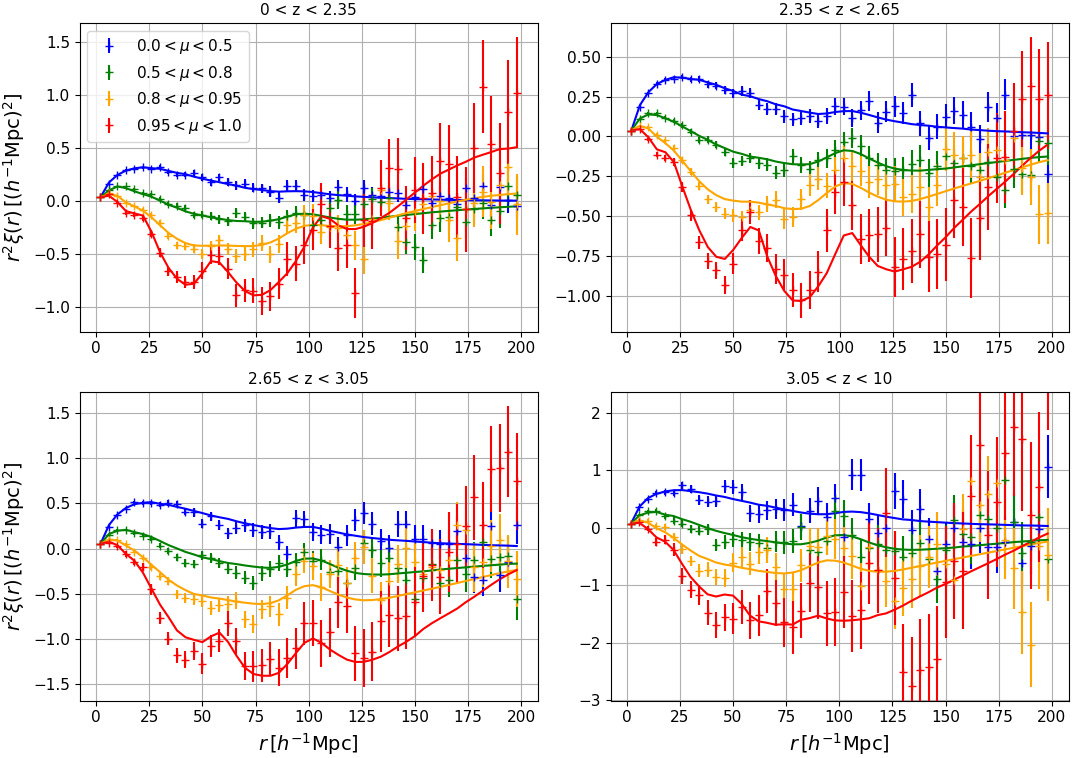
\includegraphics[scale=0.4]{dr16_4bins}
  \caption{Fonctions de corrélation \lya{}$\times$\lya{} dans chacun des bins en redshift de l'analyse. Les courbes en trait plein donne le meilleur ajustement du modèle obtenu avec \texttt{picca}. Chaque graphique correspond à un bin en redshift. Pour chacun des bins, la fonction de corrélation et l'ajustement sont montrés dans quatre bins en $\mu$.}
  \label{fig:dr16_4bins}
\end{figure}

\begin{table}[]
  \centering
  \caption{Résultats de l'ajustement fait avec \texttt{picca} des fonctions de corrélation \lya{}$\times$\lya{} calculées sur les données DR16. Chaque colonne donne le résultat de l'ajustement d'un bin en redshift. La première section du tableau donne les paramètres du modèle qui sont ajustés. La seconde donne le $\chi^2$ et le redshift effectif $z_{\mathrm{eff}}$. Le nombre de bins sur lesquels le modèle est ajusté est $N_{bin} = \num{1590}$. Le modèle comporte \num{13} paramètres libres. Enfin, la dernière section donne le biais et le biais effectif du \lya{}. Ils sont reliés aux paramètres $b_{\eta, \mathrm{Ly}\alpha}$ et $\beta_{\mathrm{Ly}\alpha}$ par les équations~\ref{eq:def_bias} et~\ref{eq:def_bias_eff}.}
  \label{tab:dr16_4bins}
  \begin{tabular}{lcccc}
    % \toprule
    % Paramètre  & $\num{0} < z < \num{2.35}$ & $\num{2.35} < z < \num{2.65}$ & $\num{2.65} < z < \num{3.05}$ & $\num{3.05} < z < \num{10}$ \\
    % \midrule
    % $\apar{}$ & 1.0626413422656635 +/- 0.06560781661781079 & 1.0188646800560925 +/- 0.041362422911403685 & 1.029148212201299 +/- 0.07242396192712802 & 1.1200171298229007 +/- 0.08091370899309824 \\
    % $\aper{}$ & 1.0632375535901253 +/- 0.10810794059323114 & 0.9652958910718991 +/- 0.057180394974236104 & 1.0159330757036005 +/- 0.05784775528375763 0.9255146850435335 +/- 0.07206257341759192 \\
    % $b_{\eta, \mathrm{Ly}\alpha}$ & -0.1795977211203897 +/- 0.005769053847991895 & -0.19377778657236358 +/- 0.00526939132784233 & -0.2236876829818197 +/- 0.008421287322167362 & -0.2928514012382003 +/- 0.018740373333761263 \\
    % $\beta_{\mathrm{Ly}\alpha}$ & 2.093809306317262 +/- 0.210449292900992 & 1.7112686242434043 +/- 0.13322965498374356 & 1.4274033068601393 +/- 0.13841133835520955 & 1.264422978848562 +/- 0.19412583530626168 \\
    % $10^3 b_{\eta, SiII(1190)}$ & -0.0018292445000232958 +/- 0.0010951582472295686 & -0.003656308599416015 +/- 0.0006752880865250276 & -0.002801629741142273 +/- 0.0010118710088140865 & 0.00036032759305010395 +/- 0.0016376260200395207 \\
    % $10^3 b_{\eta, SiII(1193)}$ & -0.004830928957010919 +/- 0.001100315153087375 & -0.0019362727878605114 +/- 0.0006919289269201215 & -0.0007847568940101366 +/- 0.0009691126424570403 & -0.002131181997407055 +/- 0.0017224737321217046 \\
    % $10^3 b_{\eta, SiII(1260)}$ & -0.003375467125024695 +/- 0.0013329581881429706 &  -0.001969961682619123 +/- 0.000795815740207674 & -0.001317200522029868 +/- 0.0010526150274975418 & 0.0008965020540008499 +/- 0.001791480805493678 \\
    % $10^3 b_{\eta, SiIII(1207)}$ &  -0.007865921480598285 +/- 0.0011034826815558326 & -0.004523595559873886 +/- 0.0007456098975624773 & -0.0021082960921853036 +/- 0.001047671905738136 & -0.0028969289782045586 +/- 0.001740041127658313 \\
    % $10^3 b_{\eta, CIV(eff)}$ & -0.004767305959965107 +/- 0.002544174250674547 & -0.005150878411363191 +/- 0.002643560029682246 & -0.005060576315171872 +/- 0.0026177990462492584 & -0.005022340903756195 +/- 0.002605282928692776 \\
    % $b_{\textsc{HCD}}$ & -0.05959772317290102 +/- 0.007001888877137152 & -0.04517388629736585 +/- 0.0060459072913988665 & -0.06651201389736294 +/- 0.010015445096663855 & -0.022781727665758256 +/- 0.021820968368492788 \\
    % $\beta_{\textsc{HCD}}$ & 0.5513755924633041 +/- 0.08641628187515504 & 0.55971852703097 +/- 0.08649826856663473 & 1.4274033068601393 +/- 0.13841133835520955 & 0.5026113732660472 +/- 0.08990286553465421 \\
    % $10^2 A_{sky}$ & 0.015852430760394755 +/- 0.0009832458229809115 & 0.008702223782589641 +/- 0.000816825935201006 & 0.007285381419552714 +/- 0.0013334299368094303 & 0.006448552548337415 +/- 0.0033839253887543966 \\
    % $\sigma_{sky}$ & 32.542936141293126 +/- 1.7910999585024947 & 31.590693919063543 +/- 2.5612829757179214 & 31.930967631996463 +/- 4.270238324140993
    % \bottomrule & 34.1693831220765 +/- 16.09450395736028 \\

    % $\apar{}$ & 1.0626413422656635 +/- 0.06560781661781079 & 1.0188646800560925 +/- 0.041362422911403685 & 1.029148212201299 +/- 0.07242396192712802 & 1.1200171298229007 +/- 0.08091370899309824 \\
    % $\aper{}$ & 1.0632375535901253 +/- 0.10810794059323114 & 0.9652958910718991 +/- 0.057180394974236104 & 1.0159330757036005 +/- 0.05784775528375763 0.9255146850435335 +/- 0.07206257341759192 \\
    % $b_{\eta, \mathrm{Ly}\alpha}$ & -0.1795977211203897 +/- 0.005769053847991895 & -0.19377778657236358 +/- 0.00526939132784233 & -0.2236876829818197 +/- 0.008421287322167362 & -0.2928514012382003 +/- 0.018740373333761263 \\
    % $\beta_{\mathrm{Ly}\alpha}$ & 2.093809306317262 +/- 0.210449292900992 & 1.7112686242434043 +/- 0.13322965498374356 & 1.4274033068601393 +/- 0.13841133835520955 & 1.264422978848562 +/- 0.19412583530626168 \\
    % $10^3 b_{\eta, SiII(1190)}$ & -1.8292445000232958 +/- 1.0951582472295686 & -3.656308599416015 +/- 0.6752880865250276 & -2.801629741142273 +/- 1.0118710088140865 & 0.36032759305010395 +/- 1.6376260200395207 \\
    % $10^3 b_{\eta, SiII(1193)}$ & -4.830928957010919 +/- 1.100315153087375 & -1.9362727878605114 +/- 0.6919289269201215 & -0.7847568940101366 +/- 0.9691126424570403 & -2.131181997407055 +/- 1.7224737321217046 \\
    % $10^3 b_{\eta, SiII(1260)}$ & -3.375467125024695 +/- 1.3329581881429706 &  -1.969961682619123 +/- 0.795815740207674 & -1.317200522029868 +/- 1.0526150274975418 & 0.8965020540008499 +/- 1.791480805493678 \\
    % $10^3 b_{\eta, SiIII(1207)}$ &  -7.865921480598285 +/- 1.1034826815558326 & -4.523595559873886 +/- 0.7456098975624773 & -2.1082960921853036 +/- 1.047671905738136 & -2.8969289782045586 +/- 1.740041127658313 \\
    % $10^3 b_{\eta, CIV(eff)}$ & -4.767305959965107 +/- 2.544174250674547 & -5.150878411363191 +/- 2.643560029682246 & -5.060576315171872 +/- 2.6177990462492584 & -5.022340903756195 +/- 2.605282928692776 \\
    % $b_{\textsc{HCD}}$ & -0.05959772317290102 +/- 0.007001888877137152 & -0.04517388629736585 +/- 0.0060459072913988665 & -0.06651201389736294 +/- 0.010015445096663855 & -0.022781727665758256 +/- 0.021820968368492788 \\
    % $\beta_{\textsc{HCD}}$ & 0.5513755924633041 +/- 0.08641628187515504 & 0.55971852703097 +/- 0.08649826856663473 & 1.4274033068601393 +/- 0.13841133835520955 & 0.5026113732660472 +/- 0.08990286553465421 \\
    % $10^2 A_{sky}$ & 1.5852430760394755 +/- 0.09832458229809115 & 0.8702223782589641 +/- 0.0816825935201006 & 0.7285381419552714 +/- 0.13334299368094303 & 0.6448552548337415 +/- 0.33839253887543966 \\
    % $\sigma_{sky}$ & 32.542936141293126 +/- 1.7910999585024947 & 31.590693919063543 +/- 2.5612829757179214 & 31.930967631996463 +/- 4.270238324140993
    % \bottomrule & 34.1693831220765 +/- 16.09450395736028 \\

%     $\apar{} $ & $ 1.063 \pm 0.066 $ & $ 1.019 \pm 0.041 $ & $ 1.029 \pm 0.072 $ & $ 1.120 \pm 0.081 $ \\
%     $\aperp{} $ & $ 1.063 \pm 0.108 $ & $ 0.965 \pm 0.057 $ & $ 1.016 \pm 0.058 $ & $ 0.926 \pm 0.072 $ \\
%     $b_{\eta, \mathrm{Ly}\alpha} $ & $ -0.1796 \pm 0.0058 $ & $ -0.1938 \pm 0.0053 $ & $ -0.2239 \pm 0.0084 $ & $ -0.2929 \pm 0.0187 $ \\
%     $\beta_{\mathrm{Ly}\alpha} $ & $ 2.094 \pm 0.210 $ & $ 1.711 \pm 0.133 $ & $ 1.427 \pm 0.138 $ & $ 1.264 \pm 0.194 $ \\
%     $10^3 b_{\eta, SiII(1190)} $ & $ -1.83 \pm 1.10 $ & $ -3.66 \pm 0.68 $ & $ -2.80 \pm 1.01 $ & $ 0.36 \pm 1.64 $ \\
%     $10^3 b_{\eta, SiII(1193)} $ & $ -4.83 \pm 1.10 $ & $ -1.94 \pm 0.69 $ & $ -0.78 \pm 0.97 $ & $ -2.13 \pm 1.72 $\\
%     $10^3 b_{\eta, SiII(1260)} $ & $ -3.38 \pm 1.33 $ & $  -1.97 \pm 0.80 $ & $ -1.32 \pm 1.05 $ & $ 0.90 \pm 1.79 $\\
%     $10^3 b_{\eta, SiIII(1207)} $ & $  -7.87 \pm 1.10 $ & $ -4.52 \pm 0.74 $ & $ -2.11 \pm 1.05 $ & $ -2.90 \pm 1.74 $\\
%     $10^3 b_{\eta, CIV(\mathrm{eff})} $ & $ -4.77 \pm 2.54 $ & $ -5.15 \pm 2.64 $ & $ -5.06 \pm 2.62 $ & $ -5.02 \pm 2.61 $\\
%     $b_{\textsc{HCD}} $ & $ -0.0596 \pm 0.0070 $ & $ -0.0452 \pm 0.0060 $ & $ -0.0665 \pm 0.0100 $ & $ -0.0228 \pm 0.0218 $\\
%     $\beta_{\textsc{HCD}} $ & $ 0.551 \pm 0.086 $ & $ 0.560 \pm 0.086 $ & $ 0.508 \pm 0.088 $ & $ 0.503 \pm 0.090 $\\
%     $10^2 A_{sky} $ & $ 1.585 \pm 0.098 $ & $ 0.870 \pm 0.082 $ & $ 0.729 \pm 0.133 $ & $ 0.645 \pm 0.338 $\\
%     $\sigma_{sky} $ & $ 32.5 \pm 1.7 $ & $ 31.6 \pm 2.6 $ & $ 31.9 \pm 4.3 $ & $ 34.2 \pm 16.1 $\\
%     \midrule
%     $\chi^2$ & 1568.33 & 1512.33 & 1680.82 & 1674.59 \\
%     \midrule
%     $b_{\mathrm{Ly}\alpha} $ & $ -0.0832 \pm -0.0065 $ & $ -0.1099 \pm -0.0063 $ & $ -0.1521 \pm -0.01025 $ & $ -0.2248 \pm -0.0230 $\\
%     $b_{\mathrm{eff}, \mathrm{Ly}\alpha} $ & $ -0.1506 \pm 0.0046 $ & $ -0.1814 \pm 0.0045 $ & $ -0.2336 \pm 0.0074 $ & $ -0.3305 \pm 0.0169 $\\
%     \bottomrule
% \toprule
% Param\`etre  & $\num{0} < z < \num{2.35}$ & $\num{2.35} < z < \num{2.65}$ & $\num{2.65} < z < \num{3.05}$ & $\num{3.05} < z < \num{10}$ \\
% \midrule
% $\apar{} $ & $ 1.063 \pm 0.066$ & $ 1.019 \pm 0.041$ & $ 1.029 \pm 0.072$ & $ 1.12 \pm 0.081$ \\
% $\aperp{} $ & $ 1.063 \pm 0.108$ & $ 0.965 \pm 0.057$ & $ 1.016 \pm 0.058$ & $ 0.926 \pm 0.072$ \\
% $b_{\eta, \mathrm{Ly}\alpha} $ & $ -0.1796 \pm 0.0058$ & $ -0.1938 \pm 0.0053$ & $ -0.2237 \pm 0.0084$ & $ -0.2929 \pm 0.0187$ \\
% $\beta_{\mathrm{Ly}\alpha} $ & $ 2.094 \pm 0.21$ & $ 1.711 \pm 0.133$ & $ 1.427 \pm 0.138$ & $ 1.265 \pm 0.194$ \\
% $10^3 b_{\eta, SiII(1190)} $ & $ -1.83 \pm 1.1$ & $ -3.66 \pm 0.68$ & $ -2.8 \pm 1.01$ & $ 0.36 \pm 1.64$ \\
% $10^3 b_{\eta, SiII(1193)} $ & $ -4.83 \pm 1.1$ & $ -1.94 \pm 0.69$ & $ -0.79 \pm 0.97$ & $ -2.13 \pm 1.72$ \\
% $10^3 b_{\eta, SiII(1260)} $ & $ -3.38 \pm 1.33$ & $ -1.97 \pm 0.8$ & $ -1.32 \pm 1.05$ & $ 0.9 \pm 1.79$ \\
% $10^3 b_{\eta, SiIII(1207)} $ & $ -7.87 \pm 1.1$ & $ -4.52 \pm 0.75$ & $ -2.11 \pm 1.05$ & $ -2.89 \pm 1.74$ \\
% $10^3 b_{\eta, CIV(\mathrm{eff})} $ & $ -4.77 \pm 2.54$ & $ -5.15 \pm 2.64$ & $ -5.06 \pm 2.62$ & $ -5.02 \pm 2.61$ \\
% $b_{\textsc{HCD}} $ & $ -0.0596 \pm 0.007$ & $ -0.0452 \pm 0.006$ & $ -0.0665 \pm 0.01$ & $ -0.0228 \pm 0.0218$ \\
% $\beta_{\textsc{HCD}} $ & $ 0.551 \pm 0.086$ & $ 0.56 \pm 0.086$ & $ 0.508 \pm 0.088$ & $ 0.502 \pm 0.09$ \\
% $10^2 A_{sky} $ & $ 1.585 \pm 0.098$ & $ 0.87 \pm 0.082$ & $ 0.729 \pm 0.133$ & $ 0.646 \pm 0.338$ \\
% $\sigma_{sky} $ & $ 32.5 \pm 1.8$ & $ 31.6 \pm 2.6$ & $ 31.9 \pm 4.3$ & $ 34.1 \pm 16.0$ \\
% \midrule
% $\chi^2$ & $ 1568 $ & $ 1512 $ & $ 1681 $ & $ 1675 $ \\
% $z_{\mathrm{eff}}$ & $ 2.136 $ & $ 2.276 $ & $ 2.551 $ & $ 2.914 $ \\
% \midrule
% $b_{\mathrm{Ly}\alpha} $ & $ -0.0832 \pm 0.0065$ & $ -0.1099 \pm 0.0063$ & $ -0.1521 \pm 0.0103$ & $ -0.2247 \pm 0.023$ \\
% $b_{\mathrm{eff}, \mathrm{Ly}\alpha} $ & $ -0.1506 \pm 0.0046$ & $ -0.1814 \pm 0.0045$ & $ -0.2336 \pm 0.0074$ & $ -0.3305 \pm 0.0168$ \\
% \bottomrule
\toprule
Param\`etre  & $\num{0} < z < \num{2.35}$ & $\num{2.35} < z < \num{2.65}$ & $\num{2.65} < z < \num{3.05}$ & $\num{3.05} < z < \num{10}$ \\
\midrule
$\apar{} $ & $ 1.063 \pm 0.066$ & $ 1.019 \pm 0.041$ & $ 1.029 \pm 0.072$ & $ 1.12 \pm 0.081$ \\
$\aperp{} $ & $ 1.063 \pm 0.108$ & $ 0.965 \pm 0.057$ & $ 1.016 \pm 0.058$ & $ 0.926 \pm 0.072$ \\
$b_{\eta, \mathrm{Ly}\alpha} $ & $ -0.1796 \pm 0.0058$ & $ -0.1938 \pm 0.0053$ & $ -0.2237 \pm 0.0084$ & $ -0.2929 \pm 0.0187$ \\
$\beta_{\mathrm{Ly}\alpha} $ & $ 2.094 \pm 0.21$ & $ 1.711 \pm 0.133$ & $ 1.427 \pm 0.138$ & $ 1.265 \pm 0.194$ \\
$10^3 b_{\eta, SiII(1190)} $ & $ -1.83 \pm 1.1$ & $ -3.66 \pm 0.68$ & $ -2.8 \pm 1.01$ & $ 0.36 \pm 1.64$ \\
$10^3 b_{\eta, SiII(1193)} $ & $ -4.83 \pm 1.1$ & $ -1.94 \pm 0.69$ & $ -0.79 \pm 0.97$ & $ -2.13 \pm 1.72$ \\
$10^3 b_{\eta, SiII(1260)} $ & $ -3.38 \pm 1.33$ & $ -1.97 \pm 0.8$ & $ -1.32 \pm 1.05$ & $ 0.9 \pm 1.79$ \\
$10^3 b_{\eta, SiIII(1207)} $ & $ -7.87 \pm 1.1$ & $ -4.52 \pm 0.75$ & $ -2.11 \pm 1.05$ & $ -2.89 \pm 1.74$ \\
$10^3 b_{\eta, CIV(\mathrm{eff})} $ & $ -4.77 \pm 2.54$ & $ -5.15 \pm 2.64$ & $ -5.06 \pm 2.62$ & $ -5.02 \pm 2.61$ \\
$b_{\textsc{HCD}} $ & $ -0.0596 \pm 0.007$ & $ -0.0452 \pm 0.006$ & $ -0.0665 \pm 0.01$ & $ -0.0228 \pm 0.0218$ \\
$\beta_{\textsc{HCD}} $ & $ 0.551 \pm 0.086$ & $ 0.56 \pm 0.086$ & $ 0.508 \pm 0.088$ & $ 0.502 \pm 0.09$ \\
$10^2 A_{sky} $ & $ 1.585 \pm 0.098$ & $ 0.87 \pm 0.082$ & $ 0.729 \pm 0.133$ & $ 0.646 \pm 0.338$ \\
$\sigma_{sky} $ & $ 32.5 \pm 1.8$ & $ 31.6 \pm 2.6$ & $ 31.9 \pm 4.3$ & $ 34.1 \pm 16.0$ \\
\midrule
$\chi^2$ & $ 1568 $ & $ 1512 $ & $ 1681 $ & $ 1675 $ \\
$z_{\mathrm{eff}}$ & $ 2.136 $ & $ 2.276 $ & $ 2.551 $ & $ 2.914 $ \\
\midrule
$b_{\mathrm{Ly}\alpha} $ & $ -0.0832 \pm 0.0065$ & $ -0.1099 \pm 0.0063$ & $ -0.1521 \pm 0.0103$ & $ -0.2247 \pm 0.023$ \\
$b_{\mathrm{eff}, \mathrm{Ly}\alpha} $ & $ -0.1506 \pm 0.0046$ & $ -0.1814 \pm 0.0045$ & $ -0.2336 \pm 0.0074$ & $ -0.3305 \pm 0.0168$ \\
\bottomrule
\end{tabular}
\end{table}


La figure~\ref{fig:dr16_4bins} présente la fonction de corrélation et le meilleur ajustement du modèle dans chacun des bins en redshift. Les différents graphiques montrent les différents bins en redshift. Dans chaque graphique, la fonction de corrélation est affichée dans plusieurs bins en $\mu$. Le tableau~\ref{tab:dr16_4bins} donne le résultat de l'ajustement dans chacun des bins en redshift. La première section du tableau donne les paramètres ajustés, la deuxième donne le redshift effectif $z_{\mathrm{eff}}$ et le $\chi^2$ obtenu. Le nombre de bins dans lesquels la fonction de corrélation est ajustée est $N_{bin} = \num{1590}$, ce qui donne un nombre de degrés de liberté $N_{d.o.f.} = \num{1590} - \num{13} = \num{1577}$. Enfin, la troisième colonne donne le biais et le biais effectif du \lya{}.
% Le biais $b_{\mathrm{Ly}\alpha} $ est obtenu comme
% \begin{equation}
%   \label{eq:def_bias}
%   b_{\mathrm{Ly}\alpha}  = \frac{b_{\eta, \mathrm{Ly}\alpha} f}{\beta_{\mathrm{Ly}\alpha}} \; .
% \end{equation}
% Le biais effectif $b_{\mathrm{eff}, \mathrm{Ly}\alpha} $ est défini comme
% \begin{equation}
%   \label{eq:def_bias_eff}
%   b_{\mathrm{eff}, \mathrm{Ly}\alpha} = b_{\mathrm{Ly}\alpha} \sqrt{1 + \frac{2}{3} \beta_{\mathrm{Ly}\alpha} + \frac{1}{5} \beta_{\mathrm{Ly}\alpha}^2} \; .
% \end{equation}
% Il est sensible à l'amplitude de la fonction de corrélation, et est moins corrélé avec $\beta_{\mathrm{Ly}\alpha}$ que l'est $b_{\eta, \mathrm{Ly}\alpha}$ ou $b_{\mathrm{Ly}\alpha}$ (\#prov doublon avec le chap4).

Une fois cette analyse produite, et toujours dans le but d'obtenir $b_{\mathrm{eff},\mathrm{Ly}\alpha}(z)$ et $\beta_{\mathrm{Ly}\alpha}(z)$ pour $\num{1.9} < z  < \num{3.6}$, nous ajustons les paramètres \lya{} mesurés dans les données par une loi de puissance. La figure~\ref{fig:bias_vs_z} donne les mesures $b_{\mathrm{eff},\mathrm{Ly}\alpha}$ et $\beta_{\mathrm{Ly}\alpha}$ dans les quatre bins en redshift, ainsi que l'ajustement fait sur ces quatres points. Pour le biais effectif, nous obtenons $b_{\mathrm{eff},\mathrm{Ly}\alpha}(z) \propto (1+z)^{\gamma}$ avec $\gamma = \num{3.474} \pm \num{0.025}$. Pour le paramètre RSD, nous obtenons $\beta_{\mathrm{Ly}\alpha}(z) \propto (1+z)^{\gamma}$ avec $\gamma = - \num{2.32} \pm \num{1.97}$. Ces deux ajustements sont utilisés comme référence pour l'ajustement des paramètres des mocks (section~\ref{sec:tuning}). Ils sont extrapolés de $z = \num{1.9}$ jusqu'à $z = \num{3.6}$.
\begin{figure}
  \centering
  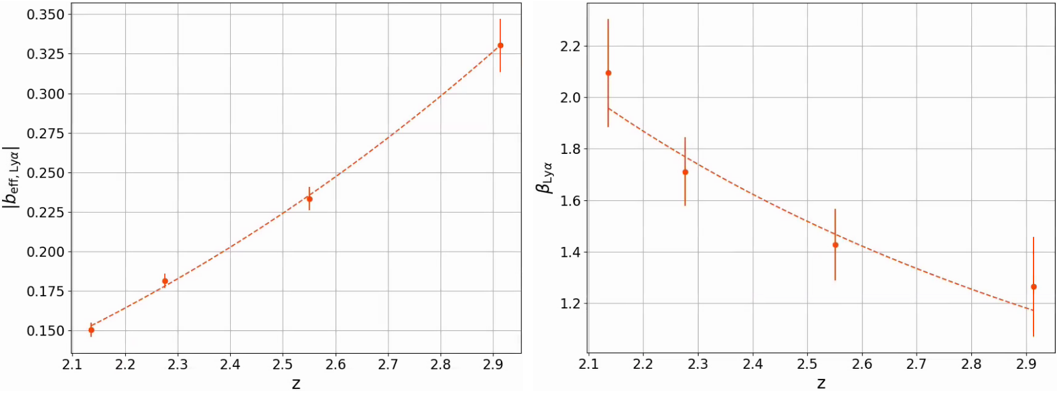
\includegraphics[scale=0.44]{bias_vs_z}
  \label{fig:bias_vs_z}
  \caption{Mesure des paramètres $b_{\mathrm{eff},\mathrm{Ly}\alpha}$ et $\beta_{\mathrm{Ly}\alpha}$ dans les données DR16. Les mesures sont faites dans quatre bins en redshift, indiquées par les points. La ligne en pointillés donne le meilleur ajustement d'une loi de puissance. Cet ajustement donne $b_{\mathrm{eff},\mathrm{Ly}\alpha}(z) \propto (1+z)^{\gamma}$ avec $\gamma = \num{3.474} \pm \num{0.025}$ et $\beta_{\mathrm{Ly}\alpha}(z) \propto (1+z)^{\gamma}$ avec $\gamma = - \num{2.32} \pm \num{1.97}$.}
\end{figure}





\subsection{Stabilité des paramètres \lya{}}
\label{subsec:stab_pars_lya}


\begin{table}[]
  \centering
  \caption{Corrélations des paramètres du modèle avec le paramètre $b_{\mathrm{eff},\mathrm{Ly}\alpha}$ lors de l'ajustement de la fonction de corrélation \lya{}$\times$\lya{}. L'ajustement est fait sur l'addition des fonctions de corrélations calculées dans chaque bin en redshift, soit l'ensemble des données DR16.}
  \label{tab:corr_bias_lya}
  \begin{tabular}{lr}
    \toprule
    Paramètre  & Corrélation avec $b_{\mathrm{eff},\mathrm{Ly}\alpha}$\\
    \midrule
    $\apar{} $ & \SI{-0}{\percent}\\
    $\aperp{} $ & \SI{1}{\percent} \\
    $b_{\eta, \mathrm{Ly}\alpha} $ & \SI{100}{\percent} \\
    $\beta_{\mathrm{Ly}\alpha} $ & \SI{-87}{\percent} \\
    $10^3 b_{\eta, SiII(1190)} $ & \SI{2}{\percent} \\
    $10^3 b_{\eta, SiII(1193)} $ & \SI{3}{\percent} \\
    $10^3 b_{\eta, SiII(1260)} $ & \SI{-1}{\percent} \\
    $10^3 b_{\eta, SiIII(1207)} $ & \SI{6}{\percent} \\
    $10^3 b_{\eta, CIV(\mathrm{eff})} $ &\SI{-7}{\percent} \\
    $b_{\textsc{HCD}} $ & \SI{48}{\percent} \\
    $\beta_{\textsc{HCD}} $ & \SI{35}{\percent} \\
    $10^2 A_{sky} $ & \SI{34}{\percent} \\
    $\sigma_{sky} $ & \SI{-10}{\percent} \\
    \bottomrule
\end{tabular}
\end{table}

\begin{table}[]
  \centering
  \caption{Corrélations des paramètres du modèle avec le paramètre $\beta_{\mathrm{Ly}\alpha}$ lors de l'ajustement de la fonction de corrélation \lya{}$\times$\lya{}. L'ajustement est fait sur l'addition des fonctions de corrélations calculées dans chaque bin en redshift, soit l'ensemble des données DR16.}
  \label{tab:corr_beta_lya}
  \begin{tabular}{lr}
    \toprule
    Paramètre  & Corrélation avec $\beta_{\mathrm{Ly}\alpha}$ \\
    \midrule
    $\apar{} $ & \SI{0}{\percent}\\
    $\aperp{} $ & \SI{-2}{\percent} \\
    $b_{\eta, \mathrm{Ly}\alpha} $ & \SI{-87}{\percent} \\
    $\beta_{\mathrm{Ly}\alpha} $ & \SI{100}{\percent} \\
    $10^3 b_{\eta, SiII(1190)} $ & \SI{-8}{\percent} \\
    $10^3 b_{\eta, SiII(1193)} $ & \SI{-6}{\percent} \\
    $10^3 b_{\eta, SiII(1260)} $ & \SI{-3}{\percent} \\
    $10^3 b_{\eta, SiIII(1207)} $ & \SI{5}{\percent} \\
    $10^3 b_{\eta, CIV(\mathrm{eff})} $ &\SI{-10}{\percent} \\
    $b_{\textsc{HCD}} $ & \SI{-75}{\percent} \\
    $\beta_{\textsc{HCD}} $ & \SI{-23}{\percent} \\
    $10^2 A_{sky} $ & \SI{-19}{\percent} \\
    $\sigma_{sky} $ & \SI{-2}{\percent} \\
    \bottomrule
\end{tabular}
\end{table}
Une fois avoir produit les ajustements présentés dans la section précédente, nous avons cherché à savoir si la mesure des paramètres \lya{} était fiable. Nous avons donc d'abord regardé la corrélation des paramètres $b_{\mathrm{eff},\mathrm{Ly}\alpha}$ et $\beta_{\mathrm{Ly}\alpha}$ avec les autres paramètres du modèle. Les tableaux~\ref{tab:corr_bias_lya} et~\ref{tab:corr_beta_lya} donnent respectivement les corrélations de $b_{\mathrm{eff},\mathrm{Ly}\alpha}$ et $\beta_{\mathrm{Ly}\alpha}$ avec les autres paramètres du modèle.
Premièrement, nous pouvons remarquer que les paramètres \lya{} sont très corrélés entre eux. Ceci vient du fait que le paramètre RSD du \lya{} est très important : le signal se trouve principalement le long de la ligne de visée. Avec peu de signal perpendiculairement à la ligne de visée, il est difficile de décorréler le biais du paramètre RSD du traceur.

Deuxièmement, les paramètres du \lya{} sont très corrélés avec ceux des HCD, notament $\beta_{\mathrm{Ly}\alpha}$ qui est corrélé à \SI{-75}{\percent} avec $b_{\textsc{HCD}}$. Ceci pose plusieurs problèmes : d'abord, la modélisation des HCD choisie dans \textcite{prov} et utilisée ici consiste à identifier puis masquer les HCD avec $\log n_{\textsc{HI}} > \num{20.3}$, les HCD non masqués étant pris en compte par le terme $F_{\textsc{HCD}}$ (voir section~\ref{subsec:model_donnees}). Cependant, l'algorithme utilisé ne possède pas une efficacité de \SI{100}{\percent} (\#prov ref papier solene). Des HCD avec une grande densité de colonne ne sont donc pas masqués.
Ces HCD produisent des absorptions intenses, non prises en compte par le terme $F_{\textsc{HCD}}$, ce qui a pour effet d'augmenter le biais du \lya{}.
De plus, le paramètre $L_{\textsc{HCD}}$ est fixé à \SI{10}{\perh\Mpc} car il est corrélé avec les autres paramètres.
Sa valeur, qui dépend de la distribution des HCD non masqués, est difficile à déterminer.
% Du fait des corrélations avec les autres paramètres, le fait de changer $L_{\textsc{HCD}}$ change la valeur de $b_{\textsc{HCD}}$.
Du fait des corrélations avec les autres paramètres, les paramètres des HCD obtenus dépendent de la valeur de $L_{\textsc{HCD}}$ choisie.
La figure~\ref{fig:bias_hcd_vs_L0} montre la dépendance de $b_{\textsc{HCD}}$ et $\beta_{\textsc{HCD}}$ avec $L_{\textsc{HCD}}$.
A cause des corrélations entre les paramètres liés aux HCD et ceux liés au \lya{}, le fait de changer $L_{\textsc{HCD}}$ change aussi les paramètres \lya{} obtenus.
La figure~\ref{fig:bias_lya_vs_L0} montre la dépendance de $b_{\mathrm{eff},\mathrm{Ly}\alpha}$ et $\beta_{\mathrm{Ly}\alpha}$ avec $L_{\textsc{HCD}}$. Ainsi, le paramètre RSD $\beta_{\mathrm{Ly}\alpha}$ est très corrélé avec $L_{\textsc{HCD}}$. Lorsque nous laissons libre $L_{\textsc{HCD}}$, en utilisant un prior gaussien centré sur \SI{10}{\perh\Mpc} et avec une largeur $\sigma = \SI{1}{\perh\Mpc}$, nous mesurons une corrélation entre $L_{\textsc{HCD}}$ et $\beta_{\mathrm{Ly}\alpha}$ de \SI{-38}{\percent}. Lorsque $L_{\textsc{HCD}}$ est laissé totalement libre, il est corrélé, en valeur absolue, à plus de \SI{85}{\percent} avec les paramètres $b_{\mathrm{eff},\mathrm{Ly}\alpha}$, $\beta_{\mathrm{Ly}\alpha}$, $b_{\textsc{HCD}}$ et $b_{\eta, SiIII(1207)}$.

Enfin, le modèle des HCD choisi influence la mesure des paramètres \lya{}. Toujours dans le but d'avoir une mesure robuste des paramètres \lya{}, nous avons essayé d'utiliser un autre modèle pour les HCD, développé par Edmond Chaussidon et Julien Guy (modèle C-G). Nous détaillons l'analyse en utilisant ce modèle dans la section~\ref{prov}.

\begin{figure}
  \centering
  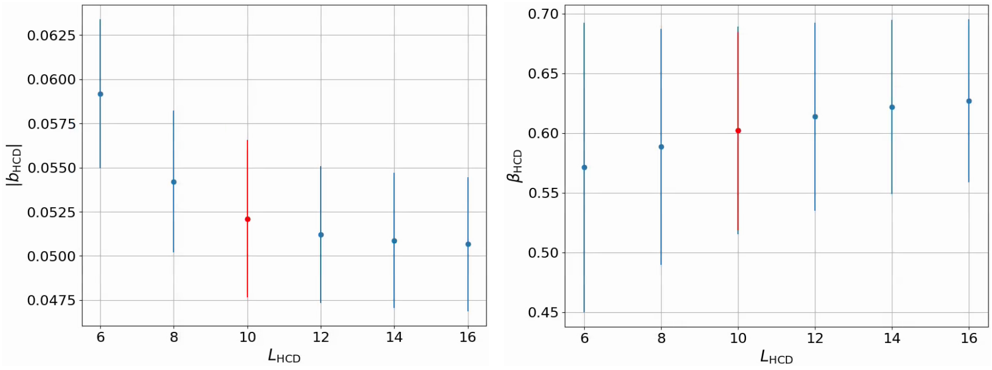
\includegraphics[scale=0.45]{bias_hcd_vs_L0}
  \caption{Evolution des mesures des paramètres $b_{\textsc{HCD}}$ et $\beta_{\textsc{HCD}}$ en fonction de la valeur $L_{\textsc{HCD}}$ choisie pour l'ajustement. Le biais des HCD est corrélé avec la valeur de $L_{\textsc{HCD}}$.}
  \label{fig:bias_hcd_vs_L0}
\end{figure}
\begin{figure}
  \centering
  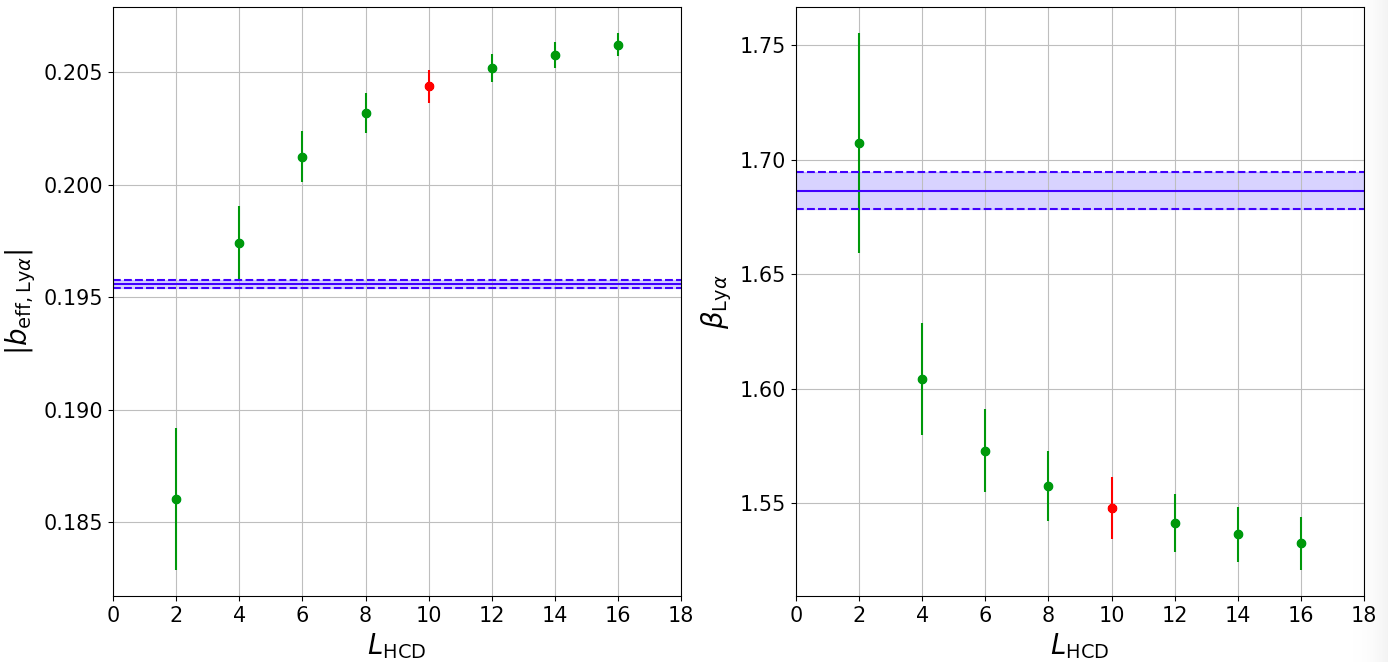
\includegraphics[scale=0.45]{bias_lya_vs_L0}
  \caption{Evolution des mesures des paramètres $b_{\mathrm{eff},\mathrm{Ly}\alpha}$ et $\beta_{\mathrm{Ly}\alpha}$ en fonction de la valeur $L_{\textsc{HCD}}$ choisie pour l'ajustement. Le paramètre RSD du \lya{} est très corrélé avec la valeur de $L_{\textsc{HCD}}$.}
  \label{fig:bias_lya_vs_L0}
\end{figure}


\section{Etude de la modélisation des HCD}

% Suite aux différents points énoncés dans la section précédente, nous avons mené une analyse sur les mocks, afin de mieux comprendre la modélisation des HCD, et d'essayer d'identifier les potentielles systématiques qui affectent la mesure des paramètres \lya{}.
Suite aux différents points énoncés dans la section précédente, nous avons étudié l'effet qu'ont les HCD sur le \lya{} dans les mocks.
En effet, les mocks sont l'outil parfait pour ce genre d'analyse : ils permettent, contrairement aux données, de connaître la quantité de \lya{} et de HCD présents, et de comparer cette quantité à ce qui est mesuré par l'ajustement.
Dans cette section, nous comparons les paramètres \lya{} mesurés dans les mocks sans HCD (raw mocks, eboss-0.0) et avec HCD (eboss-0.2 et eboss-0.3 \#prov). Nous comparons aussi les paramètres \lya{} mesurés en utilisant différentes modélisations des HCD.

\subsection{Comparaison des mocks}
Comme expliqué dans le chapitre~\ref{prov}, nous avons analysé \num{30} réalisations des raw mocks, des mocks eboss-0.0 et des mocks eboss-0.2.
Dans chacun des cas, nous ajustons le modèle sur $20 < r < \SI{180}{\perh\Mpc}$, et mesurons les paramètres du \lya{}.
La figure~\ref{fig:bias_cf} présente les mesures de ces paramètres dans chaque bin en redshift pour chacune des versions des mocks.
Nous pouvons remarquer que les valeurs des paramètres \lya{} mesurés changent selon la version des mocks.
Les paramètres mesurés dans les raw mocks sont très proches des paramètres visés, mesurés dans les données. Ceci montre que la procédure d'ajustement des paramètres des mocks que nous avons mise en place est efficace pour obtenir les bons $b_{\mathrm{eff},\mathrm{Ly}\alpha}$ et $\beta_{\mathrm{Ly}\alpha}$.

Lorsque nous comparons maintenant les valeurs de $b_{\mathrm{eff},\mathrm{Ly}\alpha}$ et $\beta_{\mathrm{Ly}\alpha}$ mesurées dans les raw mocks à celle mesurées dans les mocks eboss-0.0, nous observons un écart statistiquement significatif. L'effet sur $\beta_{\mathrm{Ly}\alpha}$ est faible, et les valeurs de $\beta_{\mathrm{Ly}\alpha}$ mesurées dans les mocks eboss-0.0 restent compatibles avec les données DR16.
Cependant, l'effet sur le biais effectif $b_{\mathrm{eff},\mathrm{Ly}\alpha}$ est important et statistiquement significatif. Cela implique que l'ajout du continuum et du bruit par quickquasars, l'ajustement du continuum ou la prise en compte des effets liés à cet ajustement par la matrice de distorsion affecte la mesure de $b_{\mathrm{eff},\mathrm{Ly}\alpha}$ et $\beta_{\mathrm{Ly}\alpha}$. Nous suspectons la matrice de distorsion de ne pas capturer tous les effets produits par l'ajustement du continuum, ce qui pourrait expliquer l'écart entre les raw mocks et les mocks eboss-0.0.

Enfin, nous observons de nouveau un écart entre les valeurs de $b_{\mathrm{eff},\mathrm{Ly}\alpha}$ et $\beta_{\mathrm{Ly}\alpha}$ mesurées dans les mocks eboss-0.0 et eboss-0.2. L'écart mesuré pour $b_{\mathrm{eff},\mathrm{Ly}\alpha}$ entre les mocks eboss-0.2 et eboss-0.0 est comparable à celui mesuré entre les mocks eboss-0.0 et les raw mocks.
L'écart mesuré sur $\beta_{\mathrm{Ly}\alpha}$ est plus important. Les valeurs obtenues dans l'ajustement des mocks eboss-0.2 ne sont pas compatibles avec celles mesurées dans les données DR16. Nous suspectons les HCD d'être à l'origine de cet écart. Comme expliqué dans la section~\ref{subsec:stab_pars_lya}, les paramètres \lya{} sont très corrélés avec ceux des HCD. Nous aurions pu par exemple choisir un $L_{\textsc{HCD}}$ plus faible dans l'ajustement des mocks eboss-0.2, ce qui aurait permis d'avoir des mesures compatibles de $\beta_{\mathrm{Ly}\alpha}$ entre les mocks eboss-0.0 et eboss-0.2 (voir figure~\ref{fig:bias_lya_vs_L0}).



\subsection{Effet du masquage des HCD}

Dans l'analyse des mocks eboss-0.2, comme pour les données, les HCD pour lesquels $\log n_{\textsc{HI}} > \num{20.3}$ sont masqués lors du calcul des $\delta_F$. Comme expliqué dans la section~\ref{subsec:stab_pars_lya}, le masquage des HCD dans les données s'effectue selon le résultat de l'agorithme d'identification, alors que dans les mocks, les HCD sont masqués à partir du ``vrai'' catalogue. Nous étudions ici l'effet du masquage à partir du catalogue produit par l'algorithme d'identification.
Pour ce faire, nous produisons l'analyse d'une réalisation de mock eboss-0.2, pour laquelle nous utilisons l'algorithme d'identification pour créer un catalogue de HCD. Le champ $\delta_F$ est calculé en masquant les HCD identifiés par l'algorithme, puis la fonction de corrélation \lya{}$\times$\lya{} est estimée dans les quatre bins en redshift utilisés jusqu'ici. Nous nommons cette analyse \emph{eboss-0.2\_finder}.
La figure~\ref{prov} présente la fonction de corrélation \lya{}$\times$\lya{} estimée à partir de la même réalisation des mocks, en version eboss-0.0, eboss-0.2 et eboss-0.2\_finder.
Les fonctions de corrélations affichées sont la moyenne des fonctions de corrélations estimées dans les quatre bins en redshift.
Dans les trois versions, le code \texttt{quickquasars} utilise les mêmes quasars pour produire les spectres synthétiques, et ajoute le même bruit à ces spectres dans les trois cas. Ceci nous permet d'avoir les mêmes fluctuations statistiques dans le calcul de la corrélation \lya{}$\times$\lya{}, et ainsi d'avoir des mesures de biais comparables.
L'effet des HCD (avec $\num{17.2} < \log n_{\textsc{HI}} < \num{20.3}$) est visible en comparant la corrélation montrée en bleu à celle montrée en rouge. Comme expliqué dans la section~\ref{subsec:model_donnees}, l'effet principal des HCD est d'augmenter le biais effectif.
De plus, le fait que l'effet des HCD soit légèrement plus important sur la corrélation de la version eboss-0.2 que sur celle de la version  eboss-0.2\_finder suggère que l'algorithme d'identification identifie correctement les HCD pour lesquels $\log n_{\textsc{HI}} > \num{20.3}$, et identifie des HCD avec $\log n_{\textsc{HI}} < \num{20.3}$ et les reconstruit avec $\log n_{\textsc{HI}} > \num{20.3}$. Ceci a pour effet de masquer des HCD qui ne possèdent pas une densité de colonne supérieure à \num{20.3}.

\begin{figure}
  \centering
  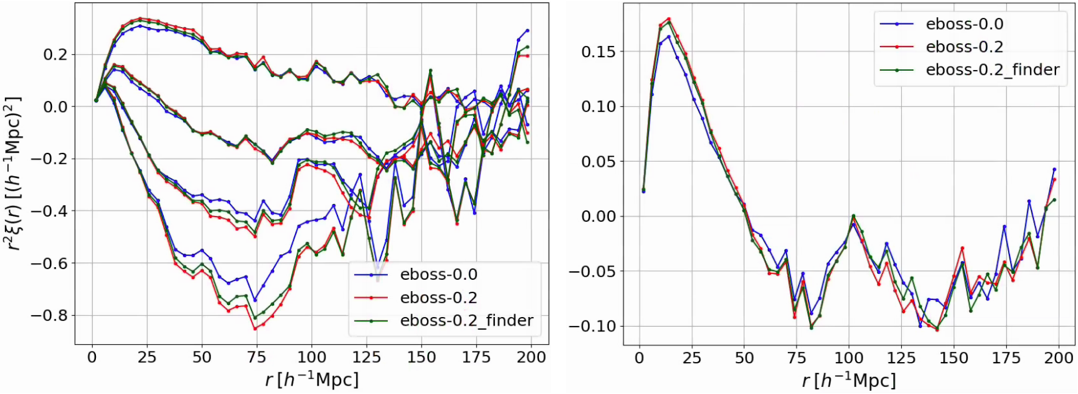
\includegraphics[scale=0.4]{cf_finder_vs_true}
  \caption{Fonctions de corrélation \lya{}$\times$\lya{} estimées à partir d'une réalisation des mocks eboss-0.0 (bleu), eboss-0.2 (rouge) et eboss-0.2\_finder (vert). La version eboss-0.2\_finder correspond aux mocks eboss-0.2, dans lesquels les HCD ont été masqués en utilisant le catalogue de HCD produit par l'algorithme d'identification.}
  \label{fig:cf_finder_vs_true}
\end{figure}

Le tableau~\ref{prov} donne les résultats des ajustements des trois corrélations présentées sur la figure~\ref{fig:cf_finder_vs_true}. La statistique d'une seule réalisation n'est pas suffisante pour identifier des potentielles systématiques. Cependant, la précision de la mesure des paramètres \lya{} dans les données DR16 étant comparable à la celle des mocks eboss-0.2, les potentielles systématiques sont inférieures à l'erreur statistique sur cette mesure.
Il serait tout de même intéressant de mener cette analyse sur un plus grand nombre de réalisations.


\begin{table}[]
  \centering
  \caption{Résultat de l'ajustement de la corrélation \lya{}$\times$\lya{} estimées à partir d'une réalisation des mocks eboss-0.0 (bleu), eboss-0.2 (rouge) et eboss-0.2\_finder (vert). La version eboss-0.2\_finder correspond aux mocks eboss-0.2, dans lesquels les HCD ont été masqués en utilisant le catalogue de HCD produit par l'algorithme d'identification.}
  \label{tab:finder_vs_true}
  \begin{tabular}{lcccc}
    \toprule
    version & $b_{\mathrm{eff},\mathrm{Ly}\alpha}$ & $\beta_{\mathrm{Ly}\alpha}$ & $b_{\textsc{HCD}}$ & $\beta_{\textsc{HCD}}$ \\
    \midrule
    eboss-0.0 & $-0.1970 \pm 0.0009$ & $ 1.641 \pm 0.039$ & & \\
    eboss-0.2 & $-0.1979 \pm 0.0038$ & $1.578 \pm 0.069$ & $-0.0201 \pm 0.0053$ & $0.499 \pm 0.090$ \\
    eboss-0.2\_finder & $-0.1951 \pm 0.0039$ & $1.592 \pm 0.074$ & $-0.0186 \pm 0.0054$ & $0.494 \pm 0.091$ \\
    \bottomrule
  \end{tabular}
\end{table}


\subsection{Modélisation alternative des HCD}

% Dans le but de tester la modélisation des HCD, nous avons ajustés les mocks et les données en utilisant une modélisation différente des HCD.
Toujours dans l'optique de tester la robustesse de la mesure des paramètres \lya{}, nous avons utilisés une modélisation des HCD différente de celle décrite dans la section~\ref{subsec:model_donnees} et utilisée jusqu'ici pour modéliser les mocks et les données.
Ce modèle est développé par Edmond Chaussidon et Julien Guy, au sein du groupe \lya{} de la collaboration DESI.
Nous faisons référence à ce modèle via le num \emph{modèle C-G}.
Ce modèle, contrairement au modèle décrit dans la section~\ref{subsec:model_donnees}, ne masque pas les HCD identifiés par l'algorithme et vérifiant $\log n_{\textsc{HI}} > 20.3$.
Ce choix est fait dans le but de s'affranchir des potentiels systématiques produites par l'utilisation de l'algorithme de détection.
Ainsi, le modèle C-G prend en compte les effets sur les corrélations \lya{}$\times$\lya{} et \lya{}$\times$QSO produits par l'ensemble des HCD dans les données.
Pour ce faire, le modèle calcule le profile de Voigt équivalent résultant



\#prov comparer les bhcd eboss-0.2 et DR16 : beaucoup plus faible dans les mocks, malgré qu'on pense avoir la bonne distribution, au moins pour nhi > 20.3.
Il faudrait multiplier le nombre de HCD par X pour que les mesures soit en accord (bhcd prop to number HCD)



% \bibliography{../source/library}
\printbibliography
\end{document}
